\documentclass[review]{elsarticle}
\usepackage{hyperref,lineno}
\usepackage{xcolor}
\usepackage[utf8]{inputenc}
\modulolinenumbers[5]

\newcommand{\memo}[2]{\textcolor{#1}{#2}}
\newcommand{\maria}[1]{\memo{red}{#1\\}}
\newcommand{\revise}[1]{\memo{blue}{#1\\}}

%\journal{Journal of Archaeological Science}


\bibliographystyle{model2-names.bst}\biboptions{authoryear}


\begin{document}

\title{The markings of the trade: exploring the patterns of olive oil production in Roman Baetica}


\begin{frontmatter}

%cambiar quizás
\begin{abstract}

The aim of this study is to detect the patterns of olive oil production that link amphora workshops and amphoric stamps. Roman provinces such as Baetica became important production and distribution centres during the Roman Empire. However, it remains under debate how this province was organized and whether it is possible to identify patterns in the olive oil market. 

Our case of study has been focused on the production processes located in Baetica province (currently Andalusia) from 1st to 3rd AD. In particular, we want to explore economic dynamics that include the production and distribution of olive oil trade. Amphoric stamps are used to identify the presence of different producer groups that might share similar stamps. To achieve this goal, we analyse a set of stamps from different workshops in Baetica province in order to detect a relation between the distribution of amphoric stamps and the economic structure in this province. Here we use methods borrowed from Ecology that allow us to identify if amphora workshops share similar amphoric stamps depending on the spatial distance. 

The analysis explores how quantitative approach provides a useful tool for the interpretation of the economic processes. Finally, results pretend to highlight the organization of Baetican olive oil production in the Roman Empire linked to the differences observed in the archaeological evidence.

\end{abstract}


\end{frontmatter}

\section{Introduction}


%primer párrafo más general---- especifico (¿dónde se ha aplicado?)
Material culture is one of the most frequent indicator of trade in the archaeological record. In archaeology, they allow us to highlight a part of mechanism of production and distribution of goods along the Mediterranean \citep{bevan_mediterranean_2014}. Particularly, the spread of these factors had an important impact during the Roman Age, when the progressive exploitation of communication networks allowed a major interaction between communities \citep{orengo_seeds_2016}. As a result, an important mechanism of production control under Roman government was created spreading by different areas attending to the richness of different places. 

Despite this issue has been widely discussed over many decades, the understanding about the production processes is still under debate, mostly due to the lack of written records. The application of different approaches combined with the archaeological evidence has allowed us partly to deal with the complexity of understanding the Roman production \citep{orengo_seeds_2016,brughmans_roman_2016,coto-sarmiento_maria_bayesian_????}.

%This paper explore--- resumir en dos líneas el objeto de estudio y definir que ha sido usado para ello dispersion of culture
This paper aims to understand the production dynamics in connection with a specific area within Roman Empire. Specifically, our work pretends to detect microeconomic processes focused on a commercial product from a specific province \citep{isaksen_network_2006}. We want to detect the pattern of olive oil production that link amphora workshops and amphoric stamps used to mark them. We focus here on exploring the economic relation between stamps and amphora production centres. To do this, an Ecology approach has been used to analyse the dispersion of stamps between amphora workshops \citep{rubio-campillo_ecology_2018}. 

% hipotesis

% Debate
 
%más específico--- olive oil
%incluir algo que enlace con roman province

\section{The amphora production in the Roman Empire}

Roman provinces such as Baetica (currently Andalusia, south Spain) became important production centres of olive oil during the Roman Empire. Olive oil was considered as the liquid gold since it was used in different aspect of the daily life as cooking, hygiene or lighting  \citep{mattingly_d.j._oil_1988}. As a consequence, the high demand of Roman provinces stimulated by the good condition of the Baetica lands allowed to develop a massive infrastructure of olive oil production. This product was distributed in large amount of amphorae along the province, mostly to supply the Roman Army and Italy \citep{blazquez_exportacion_1980}. 

The production and distribution of olive oil in this ancient province were growing exponentially during almost three centuries \citep{remesal_concierto}. As a result, thousands of amphora workshops were made to support this high demand of Roman Empire. These workshops were located along the rivers Guadalquivir and Genil, supplying from the riverine connectivity to the Mediterranean and Atlantic routes \citep{garcia_vargas_enrique_formal_2010}. 

The majority of olive oil amphorae produced in this province and shipped through the provinces belong to Dressel 20 type \citep{dressel,martin-kilcher_romischen_1994}. This amphora is commonly associated with the transportation of Baetican olive oil during the Roman Empire \citep{berni_millet_epigrafianforica_2008}. Most Dressel 20 were marked in stamps, inked in \textit{tituli picti} and incise in \textit{graffiti} with different information. However, inscriptions and \textit{tituli picti} have not enough analysed due to the fragmentation of the material or the shortage of samples \citep{aguilera_evolucion_2007,rovira_guardiola_grafitos_2007}. By contrast, stamps are the most studied in this type of amphorae. During almost three centuries, stamps were used to mark amphorae with a different chronological frequency \citep{remesal_sellar_2016}. Frequently, they were marked mainly in handles but seldom in rims and body \citep{millet_anforas_1998}. 
The information of the stamps is shown in different forms and letter content and it seems that there was not a unique criterion. Stamps are mostly formed by a code of three letters and they can appear in a abbreviated form or complete and they are known as \textit{Tria Nomina} \citep{berni_millet_amphora_1996}. 

%Many hypothesis involved the meaning of stamps. 
 There is not a general consensus about the meaning of the stamps \citep{rodriguez_baetican_1998}. It seems that stamps could have been identified as the land owner of the olive groves \citep{rodriguez_economioleicola_1977}. On the other hand, they could belong to the owner of the making amphorae workshops or even a production counting system  \citep{berni_millet_epigrafianforica_2008}. In any case, the use of these stamps became in a good proxy to define somehow the system of working in the workshops. 

%Hyphotesis
Nevertheless, some challenges remain under discussion such as how this province was organized and whether it is possible to distinguish production patterns in the olive oil trade. Our questions will be focused on the distribution of amphoric stamps. Did they follow a distribution pattern? Did stamps share the same workshop? Neither written records have been found that it could explain the economic role of Baetica province in the Roman organization. Indeed, archaeological evidence shows a highly specialized production with a long activity in a this specific area with apparently few changes \citep{remesal_anforas_2004}. 

%hipotesis: si esto es así entonces es asá
Here, therefore, this study proposes an evolutionary approach to explore the effect of Baetican olive oil production by computing of dissimilarity index. The assumption of this analysis is that closer workshops concentrate similar amphoric stamps in a specific area than the distant workshops. By contrast, if we found similar amphoric stamps in different areas between workshops then the correlation between spatial distance would not be valued.  

%resumen del paper

%hablar de las tres áreas de producción: hispalis, corduba y astigi

%this paper aims to highlight the production dynamic in connection with the proximity between amphora workshops and stamps. 

\section{Material and Methods}

\subsection{Case study}

Our case study examines the relation between the distribution of amphoric stamps and the workshops. The amphora workshops were situated in different locations in Baetica province, along the river Guadalquivir and its tributary Genil in order to detect similarities between stamps from workshops and spatial distance (see Fig.\ref{workshop})

\begin{figure}[htp]
	\centering
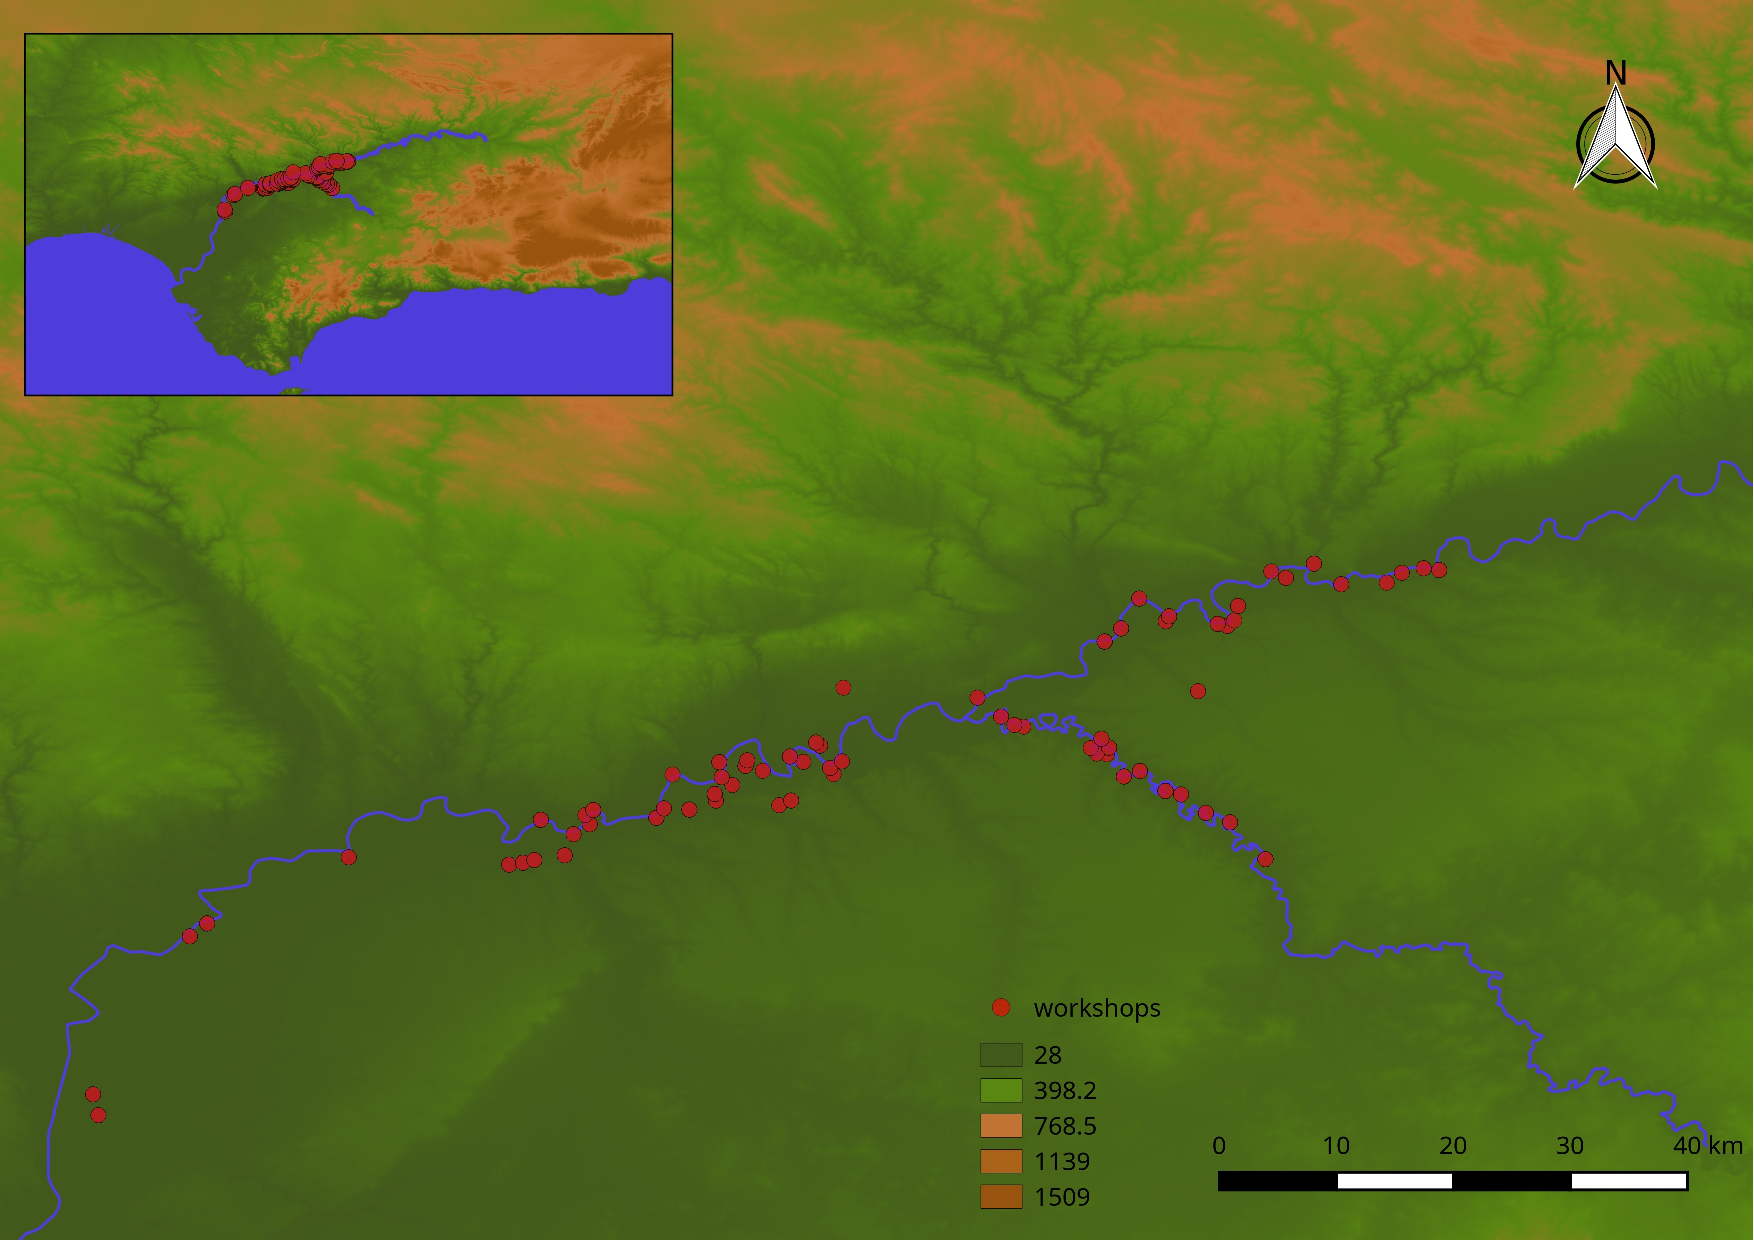
\includegraphics[width=\linewidth]{figs/workshop}
\caption{Distribution of the workshops}
\label{workshop}
\end{figure} 

The chronology in the workshops is widely diverse from the first to the third centuries AD \citep{millet_anforas_1998,rodriguez_baetican_1998,chic2005comercio}. Some stamps show a more specific chronology while the majority of them display a large activity of production that it can be difficult for specifying an accurate chronology. This could be due to two reasons; firstly, most of the workshops were partially excavated and focused on archaeological surveys in order to collect the maximum stamps as possible; secondly, Dressel 20 was produced during almost three centuries with apparently few changes. (podría citar nuestro paper por toda la face).
 
We studied a dataset of 3787 stamps collected from different Dressel 20 amphora workshops in Baetica province. The stamp database was compiled by CEIPAC database \citep{remesal_centro_2015} (see CEIPAC database here \url{http://romanopendata.eu}). However, approximately the 70 \% of stamps cannot be tested due to fragmentation or incomplete information. Consequently, we discard integrate the fragmented stamps in our dataset. We finally filter a total sample of 987 stamps comprised of 131 different stamps from 81 workshops. 

From the database, we collected the site where stamps were found and the stamp code. We also created a new column with the area of the stamps. These areas, known as \textit{conventus}, were administrative centres for territorial organization in the Roman Empire. Dressel 20 stamps were found in three different \textit{conventus}: \textit{Hispalensis} (currently Seville, hereafter Hispalis), \textit{Cordubensis} (currently C\'ordoba, hereafter Corduba) and \textit{Astigi} (currently Écija, Sevilla, hereafter Astigi) \citep{rodriguez_economioleicola_1977,chic_datos_2001,berni_millet_epigrafianforica_2008} .

The distribution of amphora stamps in different \textit{conventus} can be seen in Fig. \ref{frequency}. The majority of stamps found are concentrated in \textit{Hispalis} with 574 stamps while \textit{Corduba} and \textit{Astigi} with 267 and 146 stamps, respectively. Mostly, workshops show a homogeneity on the frequency of stamps except both La Catria and Arva that show a big amount of stamps with 29 different stamps. According to previous studies, those workshops became in most important centres of amphora production although they could have been more intensely prospected then others. \citep{arva_1997}.
 
\begin{figure}[htp]
	\centering
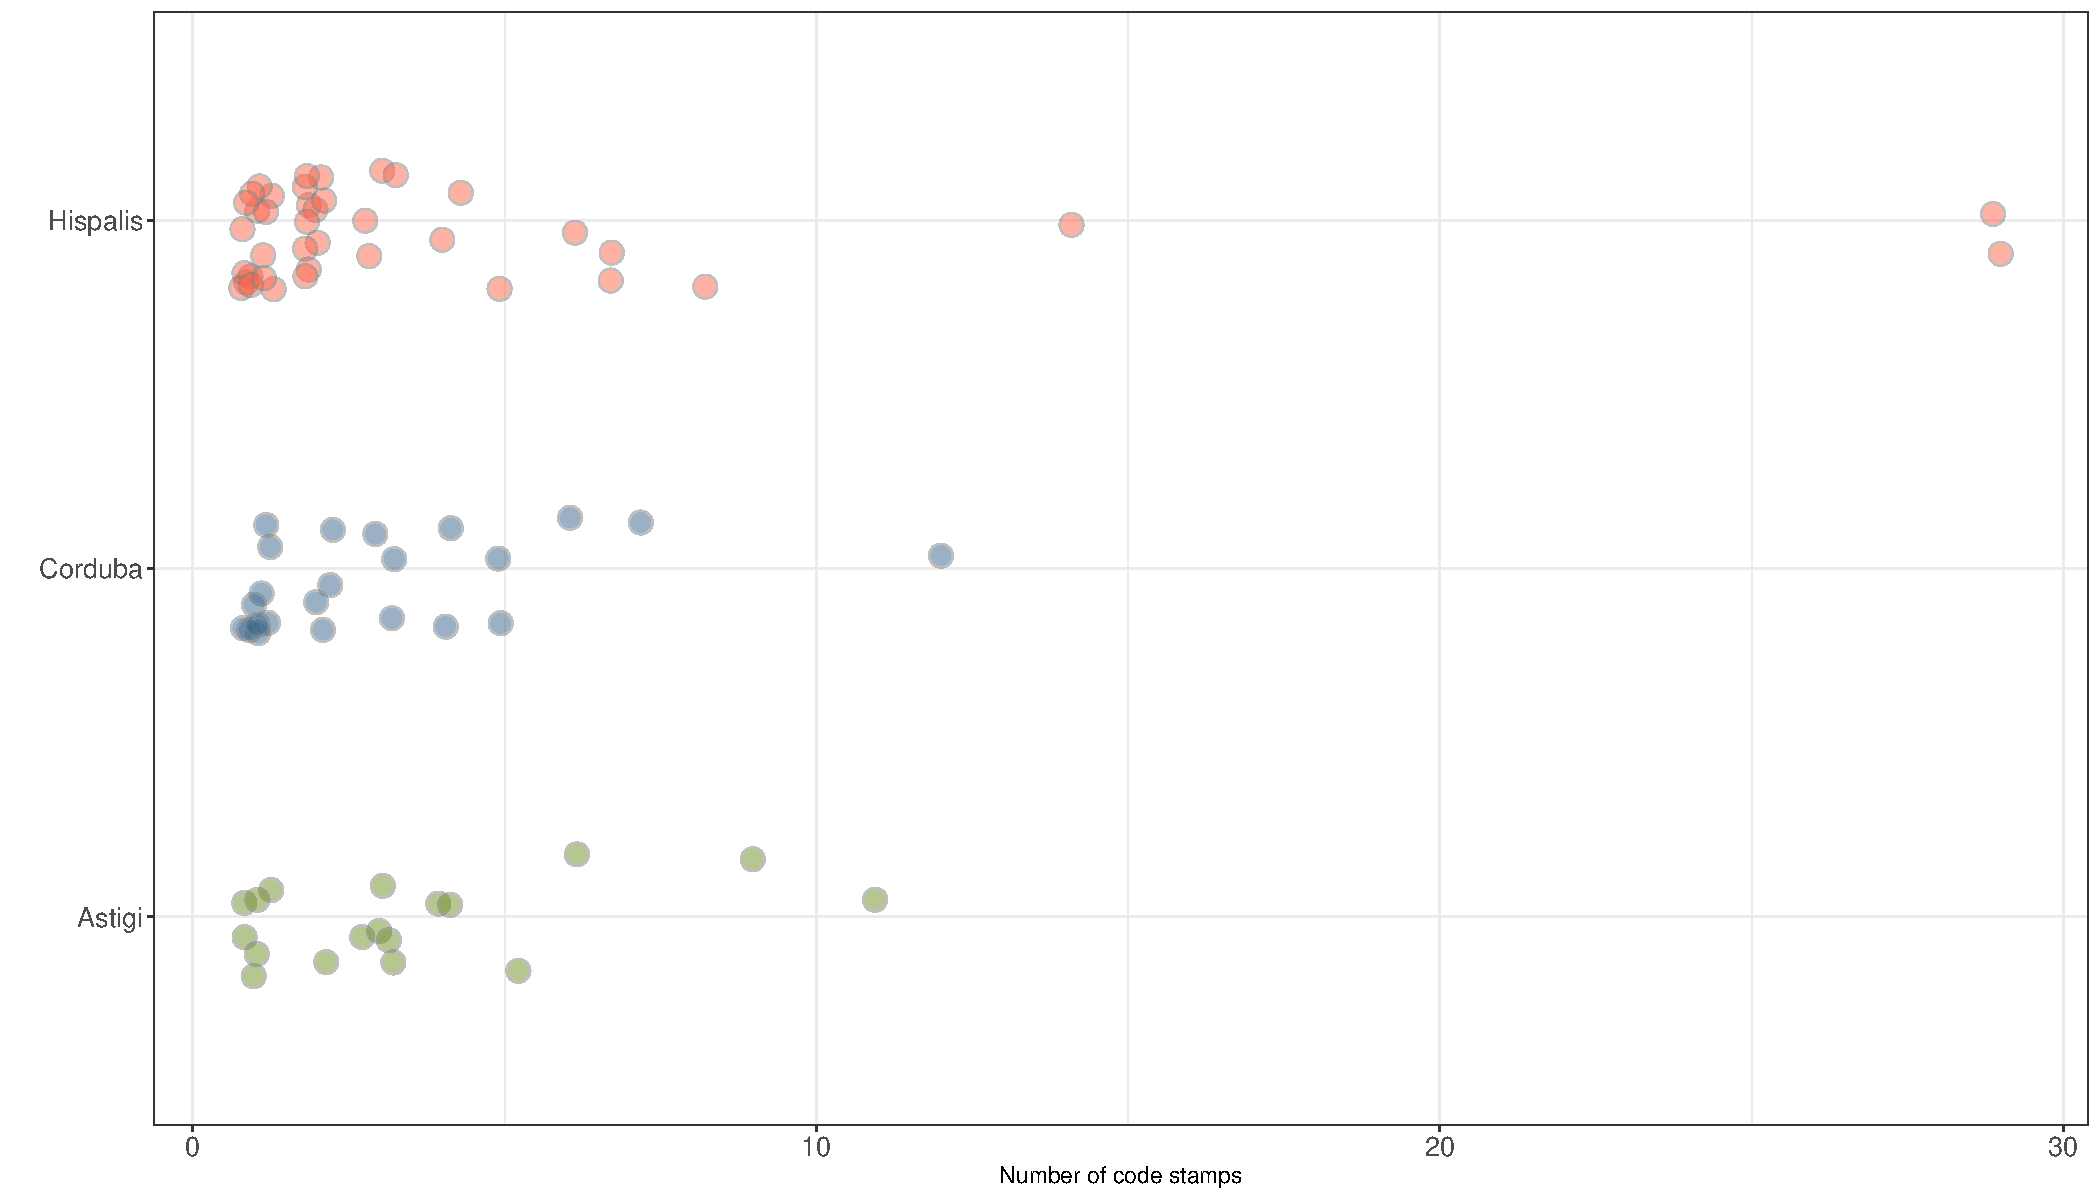
\includegraphics[width=\linewidth]{figs/frequency}
\caption{Distribution of the number of stamps for each area. Colors are represented by areas divided into Hispalis (red), Astigi (green) and Corduba (blue).}
\label{frequency}
\end{figure} 
%explicar por qué: mayor intensifación en las excavaciones quizás en sevilla

%explicar las razones del conventus no?
%aquí hablar de sellos?

%los sellos fueron marcados a partir del siglo II d.C (la economía oleícola bética Remesal) hablar de stams más concreto

%%\subsection{Jaccard distance}
%The dataset was analysed using a statistic method as Jaccard distance. This method allows to measure the dissimilarity by calculating the presence of sets (CITAR). In our case, Jaccard distance was used to compute the mutual presence of traits in the amphora stamps but it does not consider the number of absences. A comparison was done with the distance of the workshops to identify whether there was an association between stamps and spatial distance amongst workshops. 

\subsection{Quantifying the diversity}

%quizás habría que hablar también del filtrado de códigos que se hizo en python porque antes había 3783 stamps pero se filtró por el número de letras...

The approach proposed here is based on the idea of measuring the similarity between amphora workshops by quantifying similar stamps. A measure of dissimilarity has been chosen to analyse the dataset. We use the statistical technique Morisita-Horn index \citep{morisita_measuring_1959, horn_measurement_1966}. This method was performed to measure the dissimilarity between different samples of sets. Generally, it describes the dissimilarity between the system of two communities based on the idea of inverse correlation between diversity and species \citep{magurran_why_1988}.

The formula can be described as follows \citep{magurran_measuring_2013}:

\begin{equation}
D(MH) = 1- \frac{2 \sum(a_{i} \cdot b_{i})}{(d_{a} + d_{b}) \cdot (N_{a} \cdot N_{b})}
\end{equation} \\

$d_{a}$ and $d_{b}$ are given by the following equation:

\begin{equation}
d_{a} = \frac{\sum a_{i}^{2}}{N_{a}^{2}} 
\end{equation} \\

where $N_{a}$ is the total number of stamps in workshop A; $N_{b}$ is the total number of stamps in workshop B; $a_{i}$ is the number of different stamps for workshop A and $b_{i}$ is the number of different stamps for workshop B.

Considering our dataset as a non-uniform sample, this method provides a useful tool to handle large samples with different sizes and diversity \citep{wolda_similarity_1981}. Morisita-Horn index can be expressed considering 0 as total presence of similarity of stamps and 1 a totally dissimilarity between stamps. In our case, it will be calculated the number of times that one stamp appear in an amphora workshop. This method allows to bear in mind the similar number of times for each repeated stamp per workshop. If two workshops have similar stamp codes then the probability would be 0 whereas stamps codes are totally different when the results would be 1. 

%hablar sobre Horn (Morisita)hablar sobre que el sample no estaba uniforme por eso usamos el morisita horn

\section{Results}

The analysis shows that amphoric stamps could be correlated with the spatial distance. The correlation coefficients range from a minimum to a maximum. The dendrogram shown in Fig. \ref{dendro} was obtained with Morisita-Horn index. The dendrogram suggests that amphora workshops used different stamps for their production system. Nearby workshops show a similarity on the stamps while most of them seem to display different stamps roles. Additionally, groupings of similar stamps were not found in the cluster. The majority of stamp grouping was composed by no more than three workshops. Indeed workshops that shared more similar amphoric stamps belonged to the same \textit{conventus} area, such as Picachos, Cerro de los Pesebres and El Castillejo. 

\begin{figure}[htp]
	\centering
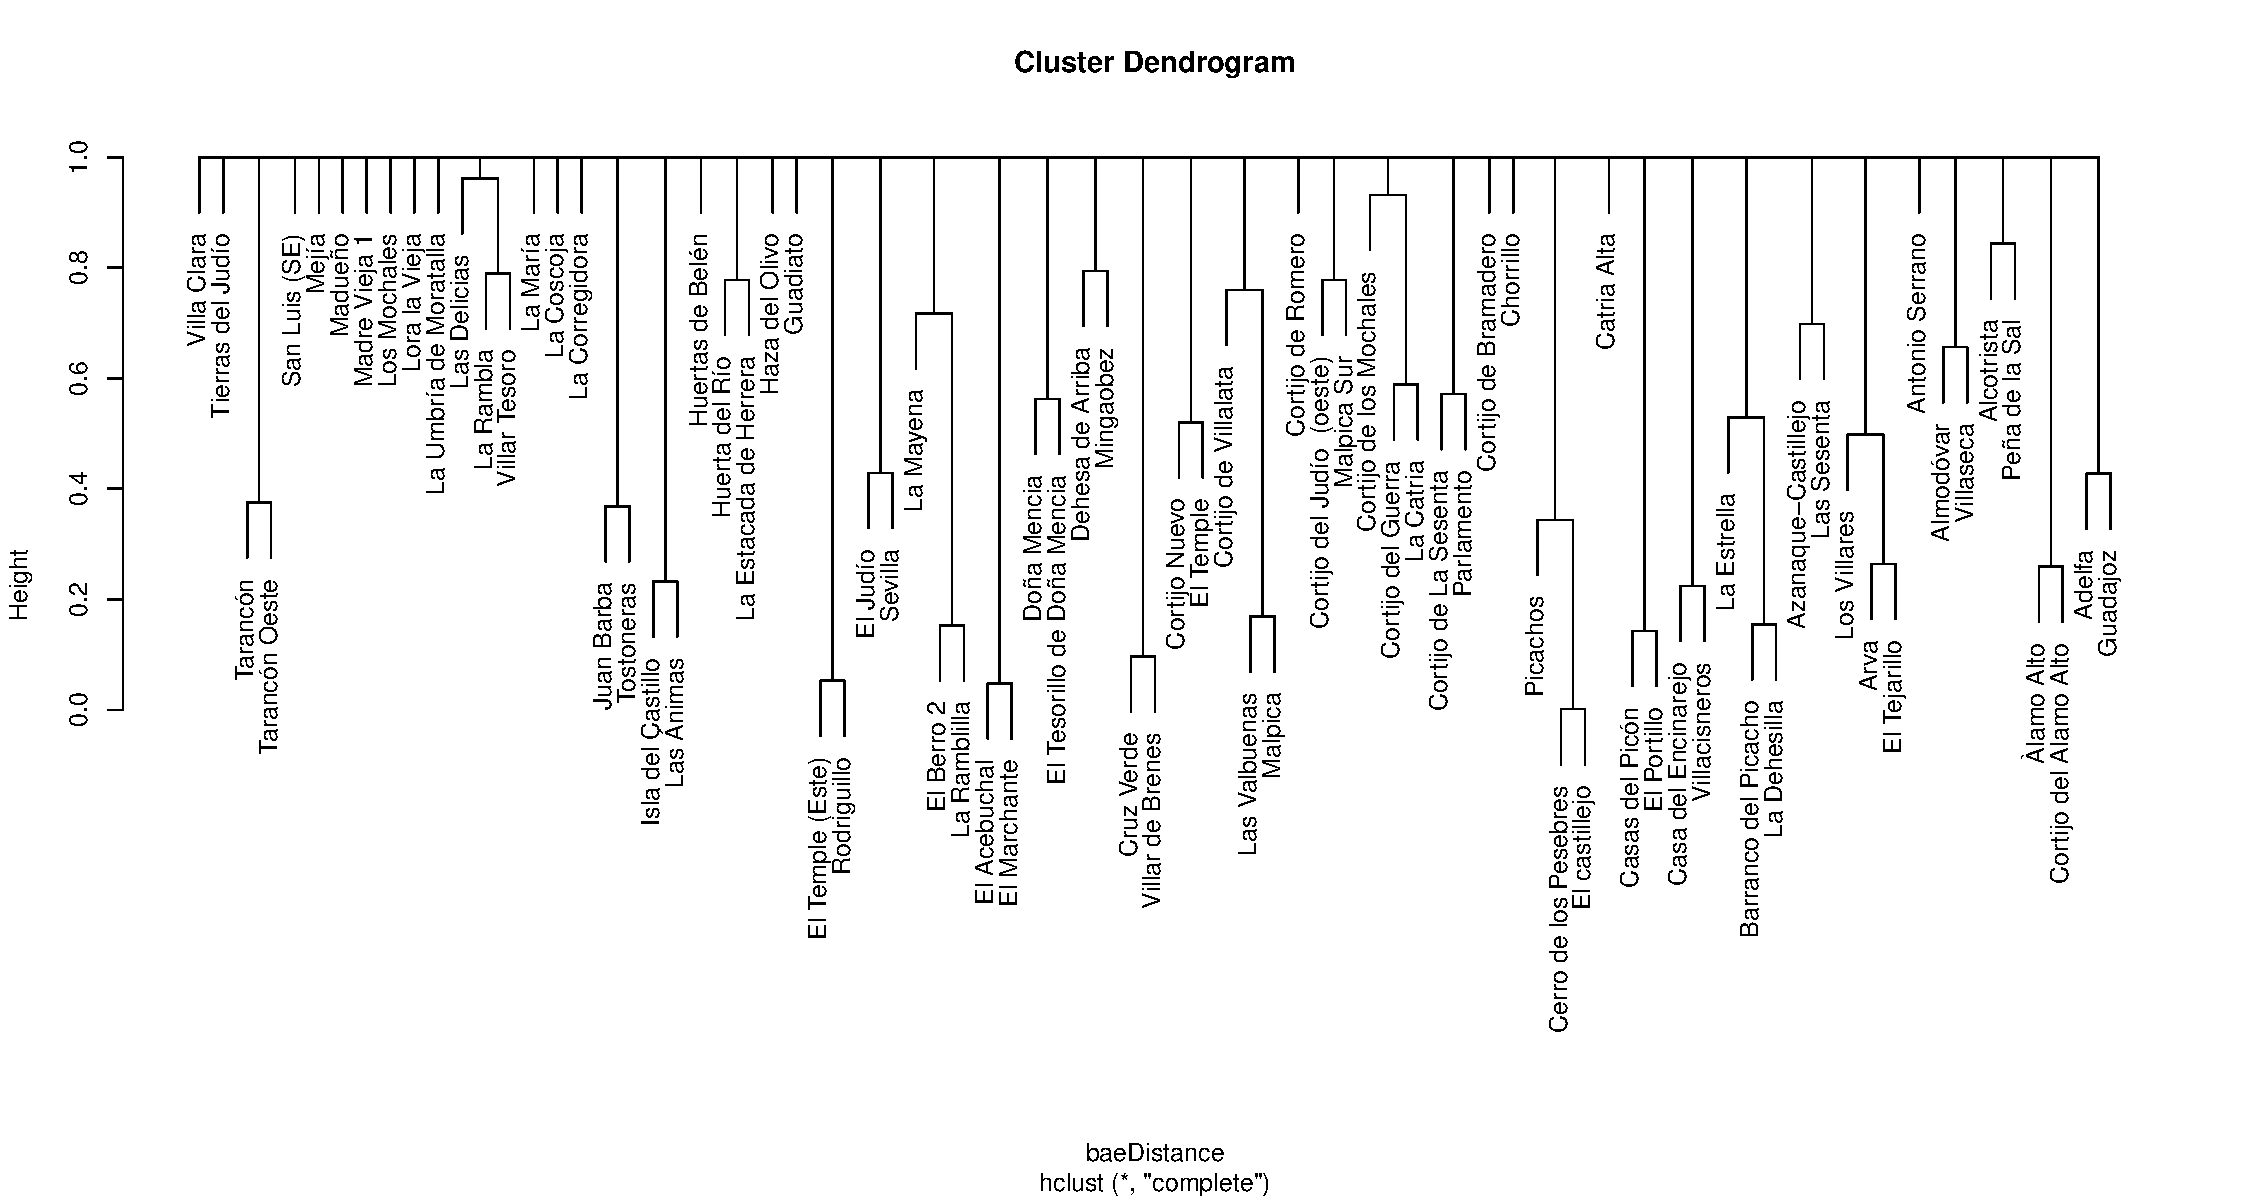
\includegraphics[width=\linewidth]{figs/dendro}
\caption{Dendrogram obtained by Morisita-Horn algorithm of different amphora workshops in Baetica area. Colours are represented by areas divided into Hispalis (red), Astigi (green) and Corduba (blue)}
\label{dendro}
\end{figure} 

%%\subsection{Jaccard distance}

%Result of Jaccard distance can be The coefficients range from x to x.The dendrogram shown in Fig. Bla bla was obtained with the Jaccard distance measure. The dendrogram suggests 


\section{Discussion and Conclusion}

%crear como una introducción

In this work, we aimed to analyse whether amphoric stamps could play an important role in the organization of the workshops along rivers. For this reason, dissimilarity index was used to detect differences among workshops and stamps. 

In our analysis, no strong relation between stamps and spatial distance have been detected in amphora workshops. The analysis suggests that there is not connection between stamps and the same amphora workshops, excluding certain exceptions when nearby workshops share the same amphoric stamp. Consequently, the majority of stamps are located in different amphora workshops and only similar stamps between closer amphora workshops were found. In any case, our results show that most similar stamps were detected in the same \textit{conventus} area. These stamps tend to share the same area of production but there is not a general relation between groups of amphora workshops and area. 

The hypothesis about groups of amphora workshops sharing the same stamps seems do not match with the results of the analysis even though there are similar stamps in closer workshops. Rather, it seems that each workshop were organized independently with different stamps. Those stamps detected in closer workshops do not move from other distant workshops. In other words, the stamps tend to keep in the same area and different stamps were located in a same amphora workshops. 

This could be defined by several factors. First, each workshop had a different organization involved to the use of stamps and they were not used in other workshops. Second, stamp similarity in closer workshops could be linked to a spatial pattern. It is more probably than closer workshops tend to share more traits than distant workshops. While the role of river was significant for the distribution of amphorae in consumption places, river connection amongst workshops does not seem show a relevancy for the distribution of stamps. Finally, the distribution of stamps could have shown some research bias. In some cases, workshops have been catalogued with different names in spite of belonging to the same workshops or being closer between each other. Additionally, most of the workshops were not widely excavated. 

%soltar aquí las hipótesis repito aquí several reasons no repetir

The results of the case study could be interpreted by several reasons. On the one hand, the use of these amphoric stamps could have been exclusively running by the owner or owners of the workshop to distinguish the amphora workshop (CITAR). This hypothesis would explain the fact that we do not find similar stamps in different workshops, however, we found different amphora stamps in the same workshops that they would be barely difficult to assign different owners. Neither a quality distinction does seem to be used to specify the value of the product \citep{callender}. On the other hand, it could be interpreted somehow a batch systematic organization. Considering that Dressel 20 was not marked in most cases, some authors point out that potters marked amphorae to prepare and distribute the commodity to be shipped \citep{berni_millet_epigrafianforica_2008}. This method would be used as an identifier to count the number of amphorae of a branch (CITAR). This method could also have served to identify different groups of potter workers working in the same amphora workshop. Potters could have marked the amphorae to distinguish different groups working in parallel \citep{li_crossbows_2014}. This it would explain wherefore why we detect different stamps in a same workshop. 
In any case, we do not have enough archaeological evidence that can validate the interpretations presented here and our results are certainly valid only with the context of our case study. 

As summary, this method presented here provides a potential tool to understand mechanisms of production based on the similarity of artefacts. This method have identified differences in the case of the amphoric production within Roman Empire. Accordingly, the results have highlighted for the interpretation of the complex economic processes connected with the archaeological evidence. 


%Dressel 20 marked in the 30-40\%

\section{Acknowledgements}
%completar 
The research was funded by European Research Council Advanced Grant EPNet (340828). We are grateful to Simon Carrignon, Juan Moros and Ignacio Morer for their useful suggestions.  
All data has been analysed and conducted in R program version 3.2.4, using the packages \textit{vegan} \citep{oksanen_vegan_2007}, \textit{ggplot2} \citep{ggplot2:_2016}. Source and code are available 


\section{References}

\bibliography{bibliotex}



\end{document}